\chapter{预备知识}

\section{公理化的集合论}

在高中我们已经学过朴素的集合论.但是,什么样的数学对象才是一个集合?描述同一群对象的集合是唯一的吗?为什么集合是无序的、不重复的?这些问题都需要通过引入公理体系来解决.

本小节不会细致深入地讲解集合论的公理化体系,因为这样会严重脱离《数学分析》的主旨.

\subsection{集合的基本性质}

先来解决不同集合的等价问题.

\begin{axiom}{外延公理}
	两个集合$A$和$B$相等当且仅当它们的元素相同.
\end{axiom}

容易验证,集合的相等是一个等价关系(后面会提到),也即它满足:
\begin{enumerate}
	\item 自反性:对于任一集合$A$都有$A=A$.
	\item 对称性:若$A=B$,则$B=A$.
	\item 传递性:若$A=B$且$B=C$,则$A=C$.
\end{enumerate}

外延公理告诉我们,描述同一群对象的任意集合都是相等的.因此,从等价类的角度来看,它的确是唯一的.

接着解决集合的无序性、不重复性问题.

\begin{axiom}{配对公理}
	对于任意集合$X,Y$,存在一个集合$Z$使得$X$和$Y$是它唯一的元素.特别地,若$X=Y$,则将$Z$视作只有唯一元素.
\end{axiom}

由配对公理,存在集合$\{ X,Y \}$和$\{ Y,X \}$,而由外延公理这两个集合是相等的,于是集合是无序的.另一方面,容易说明集合$\{ X,X \}$就等于$\{ X \}$,于是集合是不重复的.

\subsection{集合的运算}

到目前为止,我们说明了集合的一些基本性质.为了从一堆双元素集中得到更大的集合,需要引入并运算.

\begin{axiom}{并集公理}
	对于一个集合族$M$(即元素都是集合的集合),存在另一个集合$\bigcup M$,其元素恰包含所有属于$M$的集合的元素.这样的集合称作$M$的\textit{并}(union).
\end{axiom}

特别地,若$M=\{ A,B \}$,则$\bigcup M$可以记作$A \cup B$.

\begin{axiom}{分离公理}
	任意集合$A$和性质$P$都对应另一个集合$B$,其元素恰包含那些在集合$A$中而具有性质$P$的.
\end{axiom}

这实际上是在说,$B=\{ x \in A : P(x) \}$也是一个集合.

结合并集公理,马上可以定义集合族$M$的\textit{交}(intersection)为:$$\bigcap M := \{ x \in \bigcup M : \forall X,X \in M \Rightarrow x \in X \}.$$
特别地,若$M= \{ A,B \}$,则$\bigcap M$记作$A \cap B$.

顺便还能定义集合的\textit{差}(difference)和\textit{补}(complement):$$A - B := \{ x \in A : x \notin B \}.$$
如果$A$是$M$的一个子集,则定义:$$A^c := M - A.$$

另外,分离公理也表明,对任意集合$X$都存在一个不包含任何元素的子集$\varnothing _X$.由外延公理可知对任意集合$X,Y$都有$\varnothing _X = \varnothing _Y$.我们称该集合为\textit{空集}(empty set),记为$\varnothing$.

由公理体系定义的集合运算,自然具有我们在朴素集合论中学过的那些性质.

\begin{proposition}{集合运算的运算律}
	设集合$A,B,C$,集合族$\{ B_{\alpha} : \alpha \in I \}$(这里$I$是指标集). \\
	(1)交、并满足交换律,即$$A \cap B = B \cap A, \qquad A \cup B = B \cup A.$$
	(2)交、并满足结合律,即
	$$A \cap B \cap C = (A \cap B) \cap C = A \cap (B \cap C),$$
	$$A \cup B \cup C = (A \cup B) \cup C = A \cup (B \cup C).$$
	(3)交对并、并对交满足分配律,即
	$$A \cap \ssb{\bigcup_{\alpha \in I} B_\alpha} = \bigcup_{\alpha \in I} \ssb{A \cap B_{\alpha}},$$
	$$A \cup \ssb{\bigcap_{\alpha \in I} B_\alpha} = \bigcap_{\alpha \in I} \ssb{A \cup B_{\alpha}}.$$
\end{proposition}

就像中学数学所阐释的那样,补和交、并之间有一种特殊的运算律:

\begin{theorem}{de Morgan定律}
	设集合族$\{ E_{\alpha} : \alpha \in I \}$,其中$I$是指标集.则$$\ssb{\bigcup_{\alpha \in I}E_{\alpha} }^c = \bigcap_{\alpha \in I} E_{\alpha}^c,\qquad \ssb{\bigcap_{\alpha \in I}E_{\alpha} }^c = \bigcup_{\alpha \in I} E_{\alpha}^c.$$
\end{theorem}
\begin{proof}
	任取$x \in \ssb{\bigcup_{\alpha \in I}E_{\alpha} }^c$,由定义得$x \notin \bigcup_{\alpha \in I}E_{\alpha}$,所以对任意$\alpha \in I$都有$x \notin E_{\alpha}$,即对任意$\alpha \in I$都有$x \in E_{\alpha}^c$,从而可得$\ssb{\bigcup_{\alpha \in I}E_{\alpha} }^c \subseteq \bigcap_{\alpha \in I} E_{\alpha}^c$.
	
	同理可证$\ssb{\bigcup_{\alpha \in I}E_{\alpha} }^c \supseteq \bigcap_{\alpha \in I} E_{\alpha}^c$,所以$$\ssb{\bigcup_{\alpha \in I}E_{\alpha} }^c = \bigcap_{\alpha \in I} E_{\alpha}^c.$$
	
	在上式左右同取补集,立得第二个等式.
\end{proof}

最后一种构造更大集合的方式,就是枚举一个集合的所有子集.

\begin{axiom}{幂集公理}
	对任意集合$X$,总存在它的\textit{幂集}(power set)$\mathcal{P}(X)$,其元素恰为$X$的所有子集.
\end{axiom}

幂集公理允许我们构造两个集合的Cartesian积(后面会讲到).

前五个公理限制了构造新集合的方式,公理化体系下的集合论已经初步成型.接下来要介绍的三条公理,主要都是修修补补.

\subsection{无限集}

我们知道,自然数集$\mathbb{N}$理应当是无限的,然而利用前五条公理还无法说明这样的无限集存在.仿照中学学过的无限长度的数列,可以考虑利用递推的形式产生无限大的集合.更确切地说,由于现在只知道空集的存在,应该选用空集的迭代来构造无限集合.

为了让下面的公理叙述更简单,首先引入集合的后继这一概念.定义集合$X$的\textit{后继}(successor)为:$$X^{+} := X \cup \{ X \},$$
也就是说,将$X$本身放入到$X$中.

\begin{axiom}{无穷公理}
	存在集合包含空集和自身任何一个元素的后继.
\end{axiom}
\begin{remark}
	这样的集合称作是\textit{归纳的}(inductive).
\end{remark}

联系公理一至四,von Neumann提出了一种构造自然数集的方法,通过定义自然数集为所有归纳集的交集,即最小的归纳集.

要验证该交集为最小的归纳集并不难.首先注意到,任何归纳集都应包含以下元素:$$\varnothing ,\quad \varnothing ^{+}=\varnothing \cup \{ \varnothing \}=\{ \varnothing \} ,\quad (\varnothing ^{+})^{+} = \{ \varnothing \} \cup \{ \{ \varnothing \} \} = \{ \varnothing , \{ \varnothing \}\} ,\quad \cdots .$$
把这些元素组成的集合记作$N_0$.\footnote{这里的写法不太严谨,因为在用该定义证明归纳原理之前并不十分清楚$N_0$具体是什么样子,但我们知道$N_0$就是$\varnothing$导出的一切后继的集合.}由交的定义可知$$\mathbb{N} \subseteq N_0.$$
另一方面,由于$\varnothing \in \mathbb{N}$,所以$N_0 \subseteq \mathbb{N}$.从而$\mathbb{N} = N_0$.这也同时说明$\mathbb{N}$是最小的归纳集.

将$\mathbb{N}$中$\varnothing$的$n$次后继这个特征提取出来,可知$\mathbb{N}$就是一般意义上认为的自然数集(在同构\footnote{认为两个集合同构,如果在它们之间存在一个双射,后文为讲到,本质上就是这两个集合特征相同.}的意义下).

\begin{axiom}{替换公理}
	令$\mathcal{F}(x,y)$是如下命题:对于$X$中的任意元素$x_0$,存在唯一的$y_0$使得$\mathcal{F}(x_0,y_0)$成立.那么满足以下条件的$y$构成一个集合:存在$x \in X$使得$\mathcal{F}(x,y)$成立.
\end{axiom}

或者,用映射的语言来描述,替换公理就是在说:$f$是定义在集合$X$上的一个映射,那么$f$的值域也是一个集合.

替换公理在von Neumann宇宙的构造中起到一定作用,不过那会非常复杂,这里不展开讲.

\subsection{Russell悖论}

在构造无限集的过程中,可能会遇到如下问题:

\begin{definition}{Russell悖论}
	设集合$A$满足$$A = \{ x:x \notin x \}$$
	那么$A \in A$是否成立?如果成立,那么由$A$的定义可知$A \notin A$;如果不成立,那么$A$就满足$x \notin x$,从而$A \in A$.该矛盾称作Russell悖论.
\end{definition}

正是Russell悖论推翻了朴素集合论,现在我们尝试用构造新公理的方法修补这个问题.

\begin{axiom}{正则公理}
	任何非空集合$X$都存在一个元素$x$,使得$x \cap X = \varnothing$.
\end{axiom}

结合配对公理,可以证明$X \in X$这种情况是不存在的.否则,当$X$不是空集时,考虑集合$\{ X,X \}$,其中存在一个元素$x$,此时只能是$X$,使得$X \cap \{ X,X \}=\varnothing$,然而$X \in X$告诉我们$X \cap \{ X,X \} \supseteq X$,出现矛盾.当$X$是空集时,$X$内存在一个元素本就与其定义矛盾.

然而,使用正则公理只是人为禁用掉了Russell悖论出现的条件,使用减少集合论的可用范围的方式(实际上禁掉这个条件没有特别大的影响).Russell悖论不可能被最终解决.

\subsection{选择公理}

最后一条公理是选择公理,该公理可以得到许多重要的定理,然而它的否定形式与前八条公理也可相容.这种情况就类似于Euclid平面几何公理体系中的第五条,当存在的时候就是常见的Euclid几何体系,当不存在或存在其相反形式的时候就是另一套数学体系.因此,选择公理被独立于前八条之外.

\begin{axiom}{选择公理}
	对于任何由互不相交且非空的集合形成的集合族,存在另一个集合$C$,使得对该集合族中的任意元素$X$,$X \cap C$恰有一个元素.
\end{axiom}

至此,我们可以用一套公理体系来定义集合,这套体系被称作ZF(C)公理体系.

\begin{definition}{ZF(C)公理体系}
	以下八条公理组成的公理体系称作\textit{ZF公理体系}(Zermelo–Fraenkel axiom system):
	\begin{enumerate}
		\item \textit{外延公理}(axiom of extensionality)
		\item \textit{配对公理}(axiom of pairing)
		\item \textit{并集公理}(axiom of union)
		\item \textit{分离公理}(axiom of separation)
		\item \textit{幂集公理}(axiom of power set)
		\item \textit{无穷公理}(axiom of infinity)
		\item \textit{替换公理}(axiom of replacement)
		\item \textit{正则公理}(axiom of regularity)
	\end{enumerate}
	最后,再加上\textit{选择公理}(axiom of choice),就是\textit{ZFC公理体系}(Zermelo–Fraenkel axiom system with axiom of choice).
\end{definition}

\section{映射与函数}

本节内容在高中数学里已经出现过,这里简要地复习概念并做一些推广.

\begin{definition}{映射}
	\begin{itemize}
		\item 设$A$和$B$为两个集合,若对$A$中每个元素$x$,都存在$B$中唯一的元素$y$与之对应,则称此对应关系为一个\textit{映射}(map),记作$$f:A \to B,~~x \mapsto y.$$
		\item $x$在$B$中的对应元素$y$称为$x$在$f$下的\textit{象}(image),$x$称为$y$在$f$下的\textit{原象}(preimage),记作$$f(x) = y,~ x \in A.$$
		\item 集合$A$称作映射$f$的\textit{定义域}(domain);集合$B$称为映射$f$的\textit{陪域}(codomain);$A$中所有元素在$f$下的象组成的集合称为$f$的\textit{值域}(range),记作$f(A)$.
		\item 两个映射相等,当且仅当它们的定义域、对应关系、值域相同.
	\end{itemize}
\end{definition}

从集合论的视角看,一个映射其实就是确定的三元组$(A,B,f)$,其中$A$是定义域,$B$是陪域,$f$是对应关系.

映射可以有不同的表现形式.一般地,我们称从数集到数集的映射为\textit{函数}(function),将函数映射为值域的映射为\textit{泛函}(functional),从集合$A$到它本身的映射为\textit{变换}(transformation),等等.

\begin{definition}{部分映射}
	设映射$f:X \to Y$与集合$A \subseteq X$,定义$f$在$A$上的\textit{部分映射}(partial mapping)为:$$f|_A := A \to X,~~x \mapsto f(x).$$
\end{definition}
\begin{remark}
	部分映射$f_A$的值域就是$f(A)$.
\end{remark}

利用部分映射,我们可以得到一个新的映射$f$,它将包含在定义域中的集合$A$映射为其在陪域中对应的那个集合,即$$f(A) := \{ y \in Y:\exists x, (x \in A) \wedge (y=f(x)) \}.$$
在$A$就是定义域本身的时候,容易发现$f(A)$是$f$的值域.

同样地,还能定义另一个映射$f^{-1}$,它将包含在值域中的集合$B$映射为其在定义域中对应的那个集合,即$$f^{-1}(B) := \{ x \in X:f(x) \in B \}.$$

用一张图就能很好地表示上述定义(Zorich p16 Fig. 1.6):

\begin{figure}[h!]
	\centering
	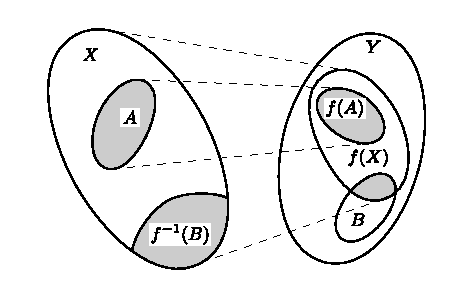
\includegraphics[width=10cm]{attachment/Acr1745354698752707434.pdf}
\end{figure}

\begin{definition}{双射}
	设映射$f:A \to B$.
	\begin{itemize}
		\item 若$A$中的每一个$x$的唯一对应$B$中的一个$f(x)$,则称$f$是\textit{单射}(injection).
		\item 若对于$B$中的每一个元素$y$,总能找到$A$中的一个$x$使得$f(x)=y$,则称$f$是\textit{满射}(surjection).
		\item 若$f$既是单射,又是满射,则称$f$是\textit{双射}(bijection)或一一映射.
	\end{itemize}
\end{definition}

\begin{definition}{映射的乘法}
    设映射$f:A \to B$,$g:B \to C$,则它们的\textit{复合映射}(composite mapping)~$gf:A \to C$定义为$$(gf)(x)=g(f(x)) \ (x \in A).$$
    注意复合运算有先后顺序.容易说明映射$gf$的定义域为$A$,值域为$C$.
\end{definition}
\begin{remark}
	为了强调复合运算,$gf$也可记作$g \circ f$.
\end{remark}

容易验证,这样的“乘法”运算满足结合律与分配律、不满足交换律.

一般将$f \circ f \circ \cdots \circ f~(n\textit{次复合})$称作$f$的$n$次迭代\footnote{严格来说,在获得自然数集的定义之前,还不能这样写.} ,记作$f^n$.

\begin{definition}{恒等映射}
	设映射$f:A \to A$.称$f$是$A$上的一个\textit{恒等映射}(identity mapping),如果$$\forall x\in A,~f(x)=x.$$
	并把$f$记作$\mathcal{I}_A$.
\end{definition}
\begin{remark}
	设映射$f : A \to B$,容易验证有$$f\mathcal{I}_A=f,\quad \mathcal{I}_Bf=f.$$
\end{remark}

下面来证明恒等映射是良定义的,即集合$A$上的所有恒等映射是相等的.假设存在两个不同的恒等映射$\mathcal{I}_1,\mathcal{I}_2$,那么由$$\mathcal{I}_1 = \mathcal{I}_1 \mathcal{I}_2 = \mathcal{I}_2,$$
可知$\mathcal{I}_1 = \mathcal{I}_2$,这与假设矛盾.

\begin{definition}{逆映射}
	设映射$f:A \to B$.称$f$是\textit{可逆的}(inverible),如果存在映射$g:B \to A$满足$$fg=\mathcal{I}_B,\quad gf=\mathcal{I}_A.$$
	特别地,称$g$为$f$的\textit{逆映射}(inverse mapping).
\end{definition}
\begin{remark}
	必须要求$g$和$f$的两种复合均等于恒等映射,否则容易出现不满足良定义的情况.
\end{remark}

逆映射也是良定义的.设映射$g_1,g_2$为$f:A \to B$的不同的逆映射,那么由$$g_1 = g_1\mathcal{I}_B = g_1fg_2 = \mathcal{I}_Ag_2 = g_2,$$
可知$g_1=g_2$,这与假设矛盾.

既然一个映射的逆映射是唯一的,我们被允许用一个符号来表示它,即$f^{-1}$.需要区分逆映射与原象集.

下面的命题刻画了何时映射是可逆的.

\begin{proposition}{可逆性等价于双射性}
	设映射$f:A \to B$,则$f$可逆当且仅当它是双射.
\end{proposition}
\begin{proof}
	\buzhou{1}必要性:设$f$可逆,即存在映射$g:B \to A$满足$fg=\mathcal{I}_B,gf=\mathcal{I}_A$.下面证明$f$是双射. \\
	设$x,y \in A$使得$f(x)=f(y)$,那么由$$x=gf(x)=gf(y)=y,$$可知$f$是单射. \\
	另一方面,设$z \in B$,由于$z=fg(z)$,这表明$B \subseteq f(A)$,故$B = f(A)$,于是$f$是满射. \\
	\buzhou{2}充分性:设$f$是单射和满射,下面证明存在映射$g:B \to A$满足$fg=\mathcal{I}_B,gf=\mathcal{I}_A$. \\
	人为地取$g$,使得$g(x)$是$A$中唯一使得$f(g(x))=x$的那个元素(唯一存在性由$f$是双射可以得到保证).按照$g$的定义,自然有$fg=\mathcal{I}_B$. \\
	另一方面,任取$x \in A$,由于$$f(gf(x)) = (fg)(f(x)) = f(x),$$并且$f$是单射,可得$gf(x)=x$,所以$gf=\mathcal{I}_A$.
\end{proof}

有些函数在定义域上并非是可逆的,然而利用部分映射可以得到其一部分的逆映射,例如三角函数.

\section{二元关系}

幂集公理现在允许我们构造两个集合的Cartesian积.

\begin{definition}{Cartesian积}
	设集合$A$和$B$,定义它们的\textit{Cartesian积}(Cartesian product, direct product)如下:$$A \times B := \{ (a,b):a \in A,b \in B \}.$$
\end{definition}
\begin{remark}
	不难发现Cartesian积是一个可逆的过程,也即任何一个在$A \times B$中的元素都可以回溯到其在$A$和$B$中的对应元素.因而Cartesian积不满足交换律和结合律.
\end{remark}
\begin{remark}
	特别地,记$A^2:=A \times A$,以及$A^n := A^{n-1} \times A~(n \geq 2)$.
\end{remark}

\begin{definition}{二元关系}
	设非空集合$S$,则称$S^2$的一个子集$\mathcal{R}$为$S$上的一个\textit{二元关系}(binary relation).若$(a,b) \in \mathcal{R}$,则称$a,b$有$\mathcal{R}$关系,记作$a\mathcal{R}b$.
\end{definition}

例如,对于集合族$M$,定义在$M$上的关系$$\boldsymbol{=} := \{ (X,Y) \in M^2 : \forall x,(x \in X) \Leftrightarrow (x \in Y) \},$$
那么集合$A,B$相等就可以表述为$A \boldsymbol{=} B$.

\subsection{等价关系}

一类在数学中很重要的关系就是等价关系,它为我们阐明了数学对象的相似性和一致的本质.

\begin{definition}{等价关系}
	设集合$S$及定义在$S$上的关系$\mathcal{R}$,如果对任意$a,b,c \in S$都有:
	\begin{enumerate}
		\item 自反性:$a\mathcal{R} a$;
		\item 对称性:$a\mathcal{R} b \Rightarrow b\mathcal{R} a$;
		\item 传递性:$a\mathcal{R} b \wedge b\mathcal{R} c \Rightarrow a\mathcal{R} c$.
	\end{enumerate}
	则称$\mathcal{R}$是$S$上的一个\textit{等价关系}(equivalence relation),记作$\sim$.
\end{definition}

把所有等价的元素放在一起,就形成了\textit{等价类}(equivalence class).具体地,定义$$[a]_{\mathcal{R}} := \{ x \in S:x\mathcal{R}a \},$$如果$\mathcal{R}$是$S$上的一个等价关系.

例如,数论中模$n$的同余关系就是一类等价关系,而模$n$的同余类就是等价类.

等价类内元素都具有同等地位,都能代表整个等价类,否则它们也不会被称作是等价的.

\begin{proposition}{等价类相等等价于代表元素等价}
	设$\mathcal{R}$是$S$上的等价关系,对于$a,b \in S$有$$[a]_{\mathcal{R}} = [b]_{\mathcal{R}} \Leftrightarrow a\mathcal{R} b.$$
\end{proposition}
\begin{proof}
	必要性显然.充分性:任取$c \in [a]_{\mathcal{R}}$,由传递性知$c \mathcal{R} b$,所以$c \in [b]_{\mathcal{R}}$,从而$[a]_{\mathcal{R}} \subseteq [b]_{\mathcal{R}}$.同理有$[b]_{\mathcal{R}} \subseteq [a]_{\mathcal{R}}$,所以$[a]_{\mathcal{R}} = [b]_{\mathcal{R}}$.
\end{proof}

还是以模$n$的同余类为例.我们发现,任何一个整数都会出现且仅会出现在一个同余类里,换句话说,所有的同余类构成类对整数集合的划分.

一般地,所有的等价类都可以构成对特定集合的划分.

\begin{definition}{集合的划分}
	对于给定集合$S$,集合族$X=\{ S_{\alpha} : \alpha \in I \}$,其中$I$是指标集.称$X$是$A$的一个\textit{划分}(partition),如果
	\begin{enumerate}
		\item $S = \bigcup_{\alpha \in I} S_{\alpha}$.
		\item $\forall \alpha \neq \beta ,~S_{\alpha} \cap S_{\beta}$.
	\end{enumerate}
\end{definition}

\begin{theorem}
	设$\mathcal{R}$是$S$上的一个等价关系,则集合族$$\{ [a]_{\mathcal{R}}:a \in S \}$$构成了$S$的一个划分.
\end{theorem}
\begin{proof}
	首先我们证明,所有$[a]_{\mathcal{R}}$的并集恰等于$S$.注意到$$\forall a \in S,~a \in [a]_{\mathcal{R}} \wedge [a]_{\mathcal{R}} \subseteq S,$$
	所以$S \subseteq \bigcup_{a \in S} [a]_{\mathcal{R}} \subseteq S$,从而$S = \bigcup_{a \in S} [a]_{\mathcal{R}}$. \\
	接着证明这些集合都是不交并.对于$[a]_{\mathcal{R}} \neq [b]_{\mathcal{R}}$,假设存在$c \in [a]_{\mathcal{R}} \cap [b]_{\mathcal{R}}$,那么$c \in [a]_{\mathcal{R}} \wedge c \in [b]_{\mathcal{R}}$,由等价关系的传递性,$a\mathcal{R}b$,与假设矛盾.于是该集合族中任意两个元素交集为空.
\end{proof}

\subsection{序关系}

类比等价关系,可以定义序关系.然而就像实数集中的$<$和$\leq$关系一样,序关系可能有两种形式:严格的和不严格的.一般地,我们更希望使用后者,因为这样可以包括更多的情况.

容易看出,上面两种情况的区别在于自反性,所以只需要把下方定义中的自反性去掉,就能得到严格偏序关系的定义.

\begin{definition}{偏序关系}
	设集合$S$及定义在$S$上的关系$\mathcal{R}$,如果对任意$a,b,c \in S$都有:
	\begin{enumerate}
		\item 自反性:$a\mathcal{R} a$;
		\item 反对称性:$a\mathcal{R} b \wedge b\mathcal{R} a \Rightarrow a=b$;
		\item 传递性:$a\mathcal{R} b \wedge b\mathcal{R} c \Rightarrow a\mathcal{R} c$.
	\end{enumerate}
	则称$\mathcal{R}$是$S$上的一个\textit{偏序关系}(partially ordered relation),记作$\preceq$.
\end{definition}

为什么偏(partially,部分地)序关系不直接称作序关系呢?这是因为,有些序关系并不能覆盖所有元素.例如对于给定集合的幂集,其中某些元素并不存在包含关系.再例如,实数间的大小关系就可以覆盖所有元素.从而引出另一个概念,全序关系:

\begin{definition}{偏序关系}
	设集合$S$及定义在$S$上的关系$\mathcal{R}$,如果对任意$a,b,c \in S$都有:
	\begin{enumerate}
		\item 反对称性:$a\mathcal{R} b \wedge b\mathcal{R} a \Rightarrow a=b$;
		\item 传递性:$a\mathcal{R} b \wedge b\mathcal{R} c \Rightarrow a\mathcal{R} c$;
		\item 完全性:$a\mathcal{R} b \vee b\mathcal{R} a$.
	\end{enumerate}
	则称$\mathcal{R}$是$S$上的一个\textit{全序关系}(totally ordered relation),同时称$S$是一个\textit{全序集}(totally ordered set).
\end{definition}
\begin{remark}
	完全性蕴含了自反性.
\end{remark}


\section{集合的基数}

高中数学中,我们学过有限集合的元素个数.从直观上看,似乎无限集合不会存在元素个数这一说法,但我们又熟知实数远比整数多,那么这种相对的元素个数比较是怎样建立的?

来考虑这样一个问题:给定两个有限集合$A,B$,如何比较它们的元素个数.最一般的想法应该是在它们之间构造一个映射$f:A \to B$,如果$f$是双射则$A,B$元素个数相等,如果是单射则$A$的元素个数不多于$B$的元素个数,如果是满射则$B$的元素个数不多于$A$的元素个数(这些用反证法容易说明).

相对应地,既然我们只需要考虑无限集合之间的相对“元素个数”多少,而不需要得到一个绝对数值,就可以仿照上方的方法定义一个无限集合的“相对元素个数”.为了引起你的直观感受,我们也将其称为“势”.这是否让你想起了电势?在接下来的内容中,你将看到集合的“势”的参考位置一般取用自然数集合.

\begin{definition}{等势集合}
	对于集合$A,B$,若存在单射$f:A \to B$,则称$A$的势小于等于$B$,记作$|A| \leq |B|$.特别地,若单射$f$同时也是一个满射,即$f$是双射,则称$A,B$\textit{等势}(equipollent),记作$|A|=|B|$.
\end{definition}

很自然地,我们可以证明集合的等势关系是一个等价关系.为了证明势的小于等于是一个全序关系,需要下方的定理:(解决这个定理需要一个巧妙的构造,看不懂也没关系,只要证明所给出的构造是双射即可)

\begin{theorem}{Schröder–Bernstein}
	给定集合$A,B$.若在$A,B$间存在两个单射$f:A \to B$与$g:B \to A$,则在它们之间也存在一个双射$h:A \to B$.
\end{theorem}
\begin{proof}
	通过以下方法构造一个映射$h:A \to B$,我们断言它就是想要的那个双射. \\
	递归地定义:$$C_0 = A - g(B),\quad C_{n+1}=g(f(C_n))~~\forall n \geq 0.$$
	并记$C = \bigcup_{n=0}^{\infty} C_n$.对任意的$x \in A$定义映射$h: A\to B$满足$$h(x) = \begin{cases}
 f(x) & \text{ if } x \in C \\
 g^{-1}(x) & \text{ if } x \notin C
\end{cases},$$并注意这里$g$的逆映射定义域被限制在了$g(B)$.由$C_0$的定义可知,若$x \notin C$,则$x \in g(B)$,所以这样的限制是合理的.接下来验证$h$是双射. \\
\buzhou{1}单射性:假设不同的$a,b$导致$h(a)=h(b)$,对以下四种情况进行讨论:$$a \in C \wedge b \in C,\qquad a \notin C \wedge b \notin C,\qquad a \in C \wedge b \notin C,\qquad a \notin C \wedge b \in C.$$
对于前两种情况,容易证明$a=b$.对于第三种情况,即有$g(f(a))=b$,而$a \in C$表明$g(f(a)) \in C$,从而与$b \notin C$矛盾.第四种情况同理. \\
综上,对任意$a,b$都有$h(a)=h(b) \Rightarrow a=b$,故$h$是单射. \\
\buzhou{2}满射性:任取$y \in B$.若$y \in f(A)$,则存在一个$x_1$使得$f(x_1)=y$,从而$h(x_1)=y$.若不然,则令$x_2=g(y)$.下面证明$x_2 \notin C$,这样就有$h(x_2)=g^{-1}(x_2)=y$: \\
假设$x_2=g(y) \in C$,那么由$C$的定义且$g$为单射,可知存在一个$x_0$使得$f(x_0)=y$,这与$y \notin f(A)$矛盾. \\
综上,对任意的$y \in B$,总能找到某个$x$使得$h(x)=y$,从而$h$是满射.
\end{proof}

由上方的定理,容易得到势的小于等于关系满足反对称性.该关系的完全性则是选择公理的推论(这里略去).再加上传递性(例如,$A,B$之间存在单射$f$,$B,C$之间存在单射$g$,则$gf$也是$A,C$间的单射),马上得到该关系是一个全序关系.

从而,我们可以利用等价类的思想刻画一个无限集合的相对元素个数.

\begin{definition}{集合的基数}
	\begin{itemize}
		\item 设集合的等势关系$\mathcal{R}$.对于集合$X$,称$[X]_{\mathcal{R}}$为其\textit{基数}(cardinal)或势,记作$\card X$.
		\item 定义$\card X = \card Y$,如果$X$与$Y$等势.
		\item 定义$\card X \leq \card Y$,如果$X$与$Y$的某个子集等势.
	\end{itemize}
\end{definition}

容易证明集合基数的小于等于关系也是一个全序关系.

关于无限集合,Cantor曾证明:(这里$(\card X < \card Y):= (\card X \leq \card Y) \wedge (\card X \neq \card Y)$.)

\begin{theorem}
	设集合$X$,则$\card X < \card \mathcal{P}(X)$.
\end{theorem}
\begin{proof}
	\boxed{\text{证法$1$}}~
	若$X$是空集,则显然成立.从而,只考虑$X$非空的情况. \\
	由于$\mathcal{P}(X)$涵盖所有$X$的一元子集,故显然有$\card X \leq \card \mathcal{P}(X)$.假设有$\card X = \card \mathcal{P}(X)$,那么存在双射$f:X \to X$. \\
	根据$f$,取$B=\{ x \in X:x \notin f(x) \}$,显然$B \in \mathcal{P}(A)$,从而存在$x$使得$f(x)=B$.此时,若$x \in B$,则由$B$的定义知$x \notin B$,矛盾;同理,若$x \notin B$,则可得$x \in B$,也矛盾. \\
	\boxed{\text{证法$2$}}~(Cantor对角线法)留到第三章揭秘.
\end{proof}

